\documentclass[a4paper, twopage]{scrreprt}

\usepackage[ngerman]{babel}
\usepackage[utf8]{inputenc}
\usepackage[backend=bibtex, style=numeric]{biblatex}
\usepackage{hyperref}
\usepackage{graphicx}
\usepackage{url}
\usepackage{caption}

\author{Samuel Hammer}
\publishers{HTBLVA Spengergasse}
\title{Vorgehensmodelle zur Projektentwicklung in der Informationstechnik}
\subtitle{Ausarbeitung für die mündl. PRE Matura 2015}

\bibliography{quellen.bib}

\begin{document}

\maketitle
\tableofcontents

\chapter{Einleitung}
\label{ch:einleitung}
IT-Projekte können je nach konkretem Anwendungsfall unterschiedlich groß bzw. komplex werden. Um unabhängig von diesen Faktoren die Übersichtlichkeit, Organisation und Struktur eines Projektes zu gewährleisten, gibt es verschiedene Vorgehensmodelle. \newline
Die existierenden Vorgehensmodelle lassen sich grob in zwei Kategorien unterteilen: 
\begin{itemize}
	\item Klassische Phasenmodelle
	\item Vorgehensmodelle zur agilen Softwareentwicklung
\end{itemize}
Abhängig vom Anwendungsfall, können verscheidene Vorgehensmodelle verschiedene Vor- und Nachteile für das Projekt haben. In der Praxis gibt es also in den seltensten Fällen ein Modell, das für die Durchführung des Projektes hundertprozentig passt. \par
\begin{figure}[h]
\centering
	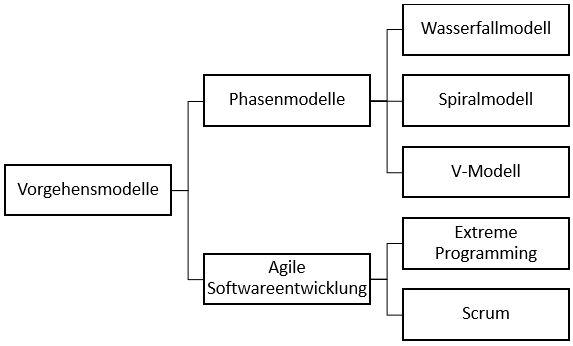
\includegraphics[scale=0.6]{Images/vorgehensmodelle_diagramm}
	\caption{Übersicht über Vorgehensmodelle\label{fig:vorgehensmodelle_diagramm}}
\end{figure}
In der folgenden Arbeit sollen die jeweiligen Vor- und Nachteile der verschiedenen Vorgehensmodelle erarbeitet und dokumentiert werden, sowie ein abschließender Vergleich inkl. Konklusion über das geeignetste Vorgehensmodell gezogen werden.

\newpage

\section{Phasenmodelle}
\label{sec:phasenmodelle}
Phasenmodelle sind "standardisierte Projektstruckturen für die Erstellung des Projektprodukts".\cite{wikipedia:projektphase}
Da allerdings nicht auf jedes Projekt die selben Phasen zutreffen, gibt es verschieden Abwandlungen. Für Softwareprojekte wird in der Regel folgende Phasenstruktur verwendet:
\begin{enumerate}
	\item Anforderungen
	\item Analyse
	\item Design
	\item Entwicklung
	\item Test
\end{enumerate}
Wenn diese verschiedenen Phasen des Projektes komplett sequentiell und unabhängig voneinander stattfinden, so spricht man vom klassischen Wasserfallmodell. (Siehe Kapitel \ref{ch:wasserfallmodell}
In der Praxis hat sich das strikte vorgehen von oben nach unten (also wie ein Wasserfall) allerdings nicht bewährt, da dieses Modell es nicht erlaubt einzelne Phasen zu wiederholen.
Für diesen Fall wurden iterative Modelle entwickelt. Hier können dann einzelne Phasen wiederholt werden falls sich beispielsweise während des Projektes die Anforderungen verändern.
\section{Agile Softwareentwicklung}
\label{sec:agile_softwareentwicklung}
Agile Softwareentwicklung gibt es seit den frühen 1990er Jahren. Mit steigender komplexität der Softwareprojekte, wurde auch der Aufwand in Bezug auf das Projektmanagement immer größer. Da klassische Phasenmodelle aufgrund ihrer geringen Flexibilität nicht mehr praktikabel waren, wurde das sogenannte "Agile Manifest" verfasst. Das Agile Manifest ist ein Werk, in dem Agile Werte definiert werden, um Softwareprojekte einfacher und besser zu gestalten. Ein Auszug aus dem Agilen Manifest besagt: \paragraph*{}
"Wir erschließen bessere Wege, Software zu entwickeln, indem wir es selbst tun und anderen dabei helfen. Durch diese Tätigkeit haben wir diese Werte zu schätzen gelernt:
\begin{itemize}
	\item \textbf{Menschen und Interaktionen} mehr als Prozesse und Werkzeuge
	\item \textbf{Funktionierende Software} mehr als umfassende Dokumentation
	\item \textbf{Zusammenarbeit mit dem Kunden} mehr als Vertragsverhandlung
	\item \textbf{Reagieren auf Veränderung} mehr als das Befolgen eines Plans
\end{itemize}
Das heißt, obwohl wir die Werte auf der rechten Seite wichtig finden, schätzen wir die Werte auf der linken Seite höher ein.“\cite{agilemanifesto}

\chapter{Wasserfallmodell}
\label{ch:wasserfallmodell}
Das Wasserfallmodell ist eines der ältesten linearen Vorgehensmodellen. Es ist nicht iterativ, d.h. wenn man nach dem Wasserfallmodell vorgeht, ist es prinzipiell nicht möglich einzelne Projektphasen zu wiederholen. Ursprünglich stammt das Wasserfallmodell aus der Bau- und Produktionsbranche. In anbetracht der Tatsache, dass zum damaligen Zeitpunkt noch kein eigenes brauchbares Modell zur Softwareentwicklung existierte, wurde das Wasserfallmodell schlicht und einfach für IT-Projekte adaptiert.
\paragraph*{}
Bei diesem Modell muss erst jede Phase abgeschlossen werden, bevor zur nächsten übergegangen werden kann. Daraus resultiert eine starke Unflexibilität, was das Wasserfallmodell vor allem bei Softwareprojekten sehr umständlich und beinahe unbrauchbar macht. Wenn beispielsweise in einem Projekt bereits mit der Programmierung begonnen wurde und der Kunde im Nachhinein eine Änderung an der Spezifikation vornehemen möchte, ist dies laut Wasserfallmodell nicht mehr möglich.
\begin{figure}[h]
\centering
	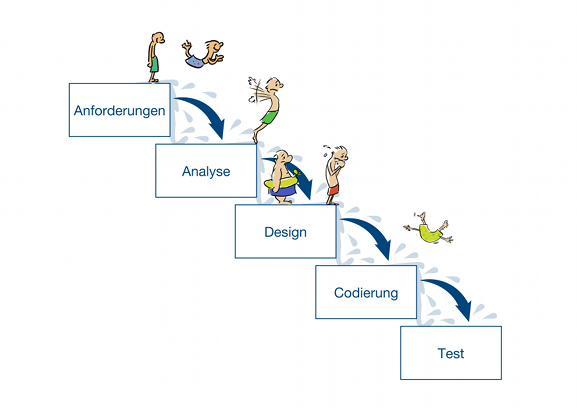
\includegraphics[scale=0.6]{Images/wasserfallmodell}
	\caption[Das Wasserfallmodell]{Das Wasserfallmodell\cite{scrumkompakt:wasserfallmodell}}
	\label{fig:wasserfallmodell}
\end{figure}
Vor allem bei langläufigen Projekten ist der Einsatz des Wasserfallmodells sehr problematisch, da sich über lange Zeiträume oft die technischen Gegebenheiten und Umgebungsbedingungen ändern können. Sollte bei weit fortgeschrittenem Projektverlauf ein Fehler in einer früheren Phase entdeckt werden, ist nicht selten ein Projektabbruch die einzige Möglichkeit den Schaden einigermaßen zu begrenzen.
\paragraph*{}
Um die oben genannten Probleme aus der Welt zu schaffen, oder zumindest zu verbessern wurde das Erweiterte Wasserfallmodell nach Royce entwickelt.
\begin{figure}[h]
\centering
	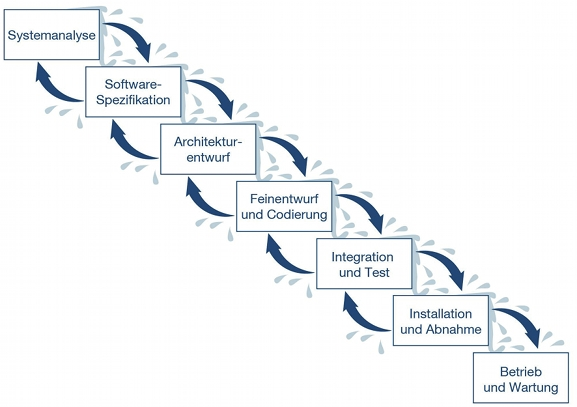
\includegraphics[scale=0.6]{Images/wasserfallmodell_erweitert}
	\caption[Erweitertes Wasserfallmodell]{Das Erweiterte Wasserfallmodell nach Royce\cite{scrumkompakt:wasserfallmodell}}
	\label{fig:wasserfallmodell_erweitert}
\end{figure}
Bei dieser Version des Wasserfallmodells sind Rücksprünge erlaubt. Nichtsdestotzotz müssen nach einem Rücksprung auf eine vorhergehende Phase, alle danach folgenden Phasen wiederholt werden. Diese Änderung verbessert das Modell zwar drastisch, allerdings werden dadurch noch lange nicht alle grundlegenden Fehler ausgemerzt.
\section{Vorteile des Wasserfallmodells}
\label{sec:wasserfallmodell_vorteile}
Da das Wasserfallmodell ein sehr altes und rudimentäres Vorgehensmodell ist, hat es, auf heutige Projekte bezogen, nicht viele Vorteile. \newline 
Ein entscheidender Vorteil ist allerdings die Einfachheit des Modells. Es lässt sich in der Praxis sehr leicht auf ein Projekt anwenden und vermittelt schnell und einfach den Eindruck von Übersicht und Kontrolle. Entgegen aller Kritik, kann das Wasserfallmodell also durchaus sinnvoll sein, solange sich das Projekt im sehr kleinen Rahmen bewegt.
\section{Nachteile des Wasserfallmodells}
\label{sec:wasserfallmodell_nachteile}
Wie bereits in Kapitel \ref{ch:wasserfallmodell} ausführlich erklärt, ist das Wasserfallmodell aufgrund der fehlenden flexibilität und der Tatsache, dass der gesamte Projektverlauf linear sein muss, in der Praxis für heutige Projekte nahezu unbrauchbar. Werden Fehler erst spät im Projektverlauf entdeckt, führt das zu sehr kostspieligen Änderungen. Des weiteren tritt durch die lange Laufzeit eines solchen Projektes, der soginannte "Return On Investment"\footnotemark erst sehr spät nach Beginn des Projektes ein.
\footnotetext{"Der Begriff Return on Investment (...) ist eine betriebswirtschaftliche Kennzahl zur Messung der Rendite einer unternehmerischen Tätigkeit, gemessen am Gewinn im Verhältnis zum eingesetzten Kapital."\cite{wikipedia:roi}}
\paragraph*{}
Auch ist es beim Wasserfallmodell oft schwierig, die einzelnen Phasen voneinander abzugrenzen. Übergänge die in der Theorie klar definiert sind, können in der Praxis oftmals eher fließend sein.

\chapter{Spiralmodell}
\label{ch:spiralmodell}
Das Spiralmodell wurde 1986 von Barry W. Boehm entwickelt. Es ist ein risikogetriebenes Vorgehensmodell, welches auf dem Wasserfallmodell basiert, sich allerdings der Idee der Iteration bedient. Im Gegensatz zum Wasserfallmodell, werden alle Phasen immer wieder wiederholt, was eine kontinuierliche Verbesserung des Projektes erlaubt. Durch die Spiralform des Modells, wird ein wiederholtes Eingreifen durch das Management in jedem Zyklus gewährleistet.
Durch die Anwendung dieses Vorgehensmodells, kann ein Projekt auch erfolgreich abgeschlossen werden, wenn sich Ziele oder Spezifikation währenddessen verändern. \par
\begin{figure}[h]
\centering
	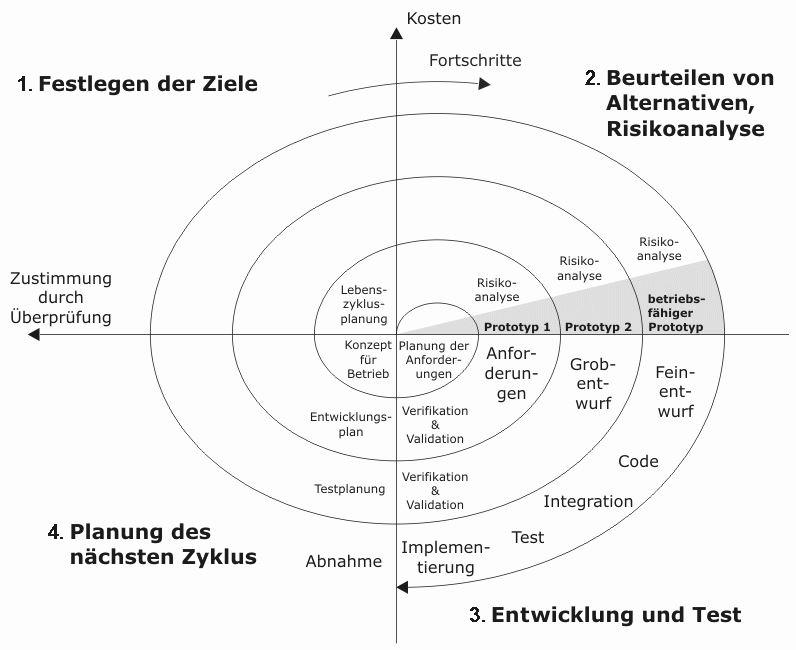
\includegraphics[scale=0.6]{Images/spiralmodell}
	\caption[Das Spiralmodell]{Das Spiralmodell\cite{wikipedia:spiralmodell}}
	\label{fig:spiralmodell}
\end{figure}
Wie in Abbildung \ref{fig:spiralmodell} zu sehen ist, bewegt sich die Linie (Zeitfortschritt) vom Ursprung aus nach außen. Jede Umdrehung um den Koordinatenursprung weist dabei einen vollendeten Zyklus auf.
Während jedes Zyklus wiederholen sich immer die selben 4 Quadrandten:
\begin{enumerate}
	\item Festlegung der Ziele
	\item Beurteilen von Alternativen und Risikoanalyse
	\item Entwicklung und Test
	\item Planung des nächsten Zyklus
\end{enumerate}
Ein Punkt, in welchem sich das Spiralmodell wesentlich vom Wasserfallmodell unterscheidet, ist die Risikobetrachtung. Zunächst werden Risiken analysiert und bewertet. In weiterer Folge wird versucht das gefährlichste Risiko zu identifizieren und zu beseitigen.
Durch die Spiralform, wird diese Risikoanalyse zyklisch wiederholt. Daher können neu auftretende Risiken in der nächsten Iteration wieder erkannt und beseitigt werden. Scheitert die Risikobeseitigung in irgendeinem Zyklus, so gilt das Projekt als gescheitert. Sind am Ende des Projektes alle Risiken beseitigt und das Produkt einwandfrei, so wird das Projekt erfolgreich abgeschlossen betrachtet.
\paragraph*{}
Eine zentrale Rolle beim Spiralmodell spielt auch die Erstellung von Prototypen. Durch die wiederholte Erstellung bzw. Erneuerung des Prototypen, können Risiken frühzeitig erkannt werden. Der Prototyp wird im Laufe des Projektes kontinuierlich weiterentwickelt, sodass dieser bis zum finalen Produkt immer weiter verfeinert wird.
\section{Vorteile des Spiralmodells}
\label{sec:spiralmodell_vortile}
Ein wesentlicher Vorteil des Spiralmodells im Vergleich mit anderen Vorgehensmodellen, ist die Tatsache, dass es risikogetrieben ist. Durch die regelmäßigen Risikoanalysen können etwaige Fehler schon im Vorhinein vermieden werden, was im Endeffekt sowohl Kosten-, als auch Zeitsparend ist. Auch die Tatsache, dass man durch das Prototyping schon sehr früh ein vorzeigbares Produkt zur Verfügung hat, macht das Spiralmodell zu einem brauchbaren Werkzeug für die Entwicklung von Softwareprojekten.

\section{Nachteile des Spiralmodells}
\label{sec:spiralmodell_nachteile}
Einer der zentralen Aspekte, welche das Spiralmodell ausmachen, ist gleichzeitig ein großer Nachteil; der Prototyp. Werden beim ersten Prototyp Fehler im Design gemacht, so ist es im Nachhinein schwierig diese noch zu beheben und es besteht die Gefahr, dass das Endprodukt nicht zufriedenstellend ist. 
Durch die Komplexität und, immer wiederkehrenden Risikoanalysen und den fortlaufenden Prototypen, ist das Spiralmodell auch mit einem verhälnismäßig sehr hohen Managementaufwand verbunden.


\chapter{V-Modell}
\label{ch:vmodell}
Das V-modell ist ein weiteres, auf dem Wasserfallmodell aufbauendes, Vorgehensmodell in der Softwareentwicklung. Das Projekt wird bei diesem Modell in Phasen aufgeteilt, daher zählt es ebenfalls zu den oben beschriebenen Phasenmodellen. (Siehe Kapitel \ref{sec:phasenmodelle}) Da das V-Modell allerdings neben Entwicklungsphasen auch Phasen zur Qualitätssicherung enthält, unterscheided es sich deutlich von anderen Phasenmodellen, wie dem Wasserfall- oder Spiralmodell. \par
\begin{figure}[h]
\centering
	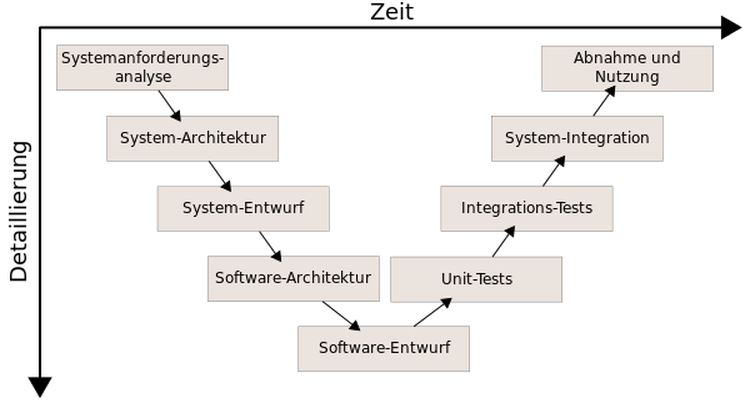
\includegraphics[scale=0.6]{Images/vmodell}
	\caption[Das V-Modell]{Das V-Modell\cite{wikipedia:vmodell}}
	\label{fig:vmodell}
\end{figure}
Wie beim Wasserfallmodell, ist das Ergebnis einer Phase eine bindende Vorgabe für die nächsttiefere bzw. nächsthöhere Projektphase. Den Entwicklungsphasen auf der linken Seite stehen die jeweils zugehörigen Testphasen auf der rechten Seite gegenüber. Durch diese Gegenüberstellung wird eine sehr hohe Testabdeckung gewährleistet, da zu jeder Entwicklungsphase genau eine Testphase gehört.
\section{Vorteile des V-Modells}
\label{sec:vmodell_vorteile}
Das V-Modell ist ein äußerst umfassendes Vorgehensmodell. Es integriert viele Aspekte des Entwicklungsprozesses und ist daher leicht erweiterbar und anpassbar. Durch die klare Struktur der Phasen ist das Modell leicht verständlich und lässt sich sehr einfach auf ein Softwareprojekt anwenden.


\section{Nachteile des V-Modells}
\label{sec:vmodell_nachteile}
Ein entscheidender Nachteil des V-Modells ist, dass es zu allgemein und generisch ist, um es auf hochkomplexe Softwareprojekte anzuwenden. Obwohl es sehr einfach verständlich ist, ist es nicht für Projekte im kleinen Rahmen geeignet, da diese meist nicht über die notwendigen Ressourcen verfügen die vorgegebenen Phasen auch einzuhalten.


\chapter{Extreme Programming}
\label{ch:extremeprogramming}
Extreme Programming\footnote{In weiterer Folge nur noch als XP bezeichnet} ist ein agiles Vorgehensmodell in der Softwareentwicklung, bei dem das Lösen von konkreten programmiertechnischen Aufgaben im Vordergrund steht. Dabei kommt der Formalen Komponente des Projektes weniger Bedeutung zu, was XP zu einer eher umstrittenen Methode macht.
\paragraph*{}
Das Ziel von XP ist es, das Produkt nicht vollständig zu einem späteren Zeitpunkt in der Zukunft auszuliefern, sondern viel mehr die Features genau dann auszuliefern, wenn der Kunde sie benötigt. Es werden von Anfang an Tests durhgeführt, was ein konstantes Feedback gewährleistet und dem Team so ermöglicht Fehler früh zu erkennen und zu beheben. Auch die Kommunikation mit dem Kunden spielt eine zentrale Rolle bei XP, so soll möglichst schnell auf Kundenwünsche oder etwaige Change Requests reagiert werden.
\paragraph*{}
XP definiert fünf zentrale Werte, welche zur erfolgreichen Ausführung eines Softwareprojektes führen sollen:
\begin{itemize}
	\item Einfachheit
	\item Kommunikation
	\item Feedback
	\item Respekt
	\item Mut
\end{itemize}
Das sind abstrakte Werte, die als Orientierung für alle Beteiligten am Projekt gelten.
\paragraph*{}
Des Weiteren gibt es 14 Prinzipien, die eine Brücke zwischen den Abstrakten Werten von XP und konkret annwendbaren Praktiken bilden sollen. Diese sind: 
\begin{center}
\textbf{Menschlichkeit, Wirtschaftlichkeit, Beidseitiger Vorteil, Selbstgleichheit, Verbesserungen, Vielfältigkeit, Reflexion, Lauf, Gelegenheiten wahrnehmen, Redundanzen vermeiden, Fehlschläge hinnehmen, Qualität, Kleine Schritte und Akzeptierte Verantwortung.}\footnote{Alle sinngemäß übersetzt}
\end{center}
Auf diese Prinzipien wird bei der Verwendung von XP viel Wert gelegt. Sie müssen auf jedenfall beachtet und bei der Entwicklung berücksichtigt werden.
\paragraph*{}
All diese abstrakten Werte und Prinzipien bringen allerdings wenig, wenn sie nicht in konkreten Praktiken umgesetzt werden. Daher wurden für XP einige Praktiken, sozusagen "best practices", definiert, die in der Realität der Softwareentwicklung angewendet werden können.
\section{XP Praktiken}
\label{sec:xp_praktiken}

\subsection{Pair-Programming}
\label{subsec:pairprogramming}
Beim Pair-Programming arbeiten immer zwei Programmierer gleichzeitig an einem konkreten Problem. Dabei ist einer derjenige der tatsächlich Programmiert (der "Driver") während der Andere eine Kontrollfunktion innehat bzw. einen gesamtüberblick über den geschriebenen Code haben sollte (der "Partner"). Dadurch wird der Wissenstransfer gefördert und Anfänger können sich leichter in ein Projekt einarbeiten. Des Weiteren wird die Fehlerdichte erheblich verringert, da ein ständiges Code Review stattfindet.
\subsection{Kollektives Eigentum}
Es soll verhindert werden, dass einzelne Programmierer einen Teil des Projekts als ihr Eigentum ansehen. Daher werden konkrete Aufgabenstellungen zuerst an das gesamte Team gestellt. Durch Pair-Programming wechselnde Aufgabengebiete, soll dies verhindert werden.
\subsection{Permanente Integration}
Es sollen einzelne Komponenten, and denen unter Umständen separat voneinander entwickelt wird, regelmäßig und kontinuierlich zu einem Großen Gesamtsystem zusammengefügt werden. Dadurch sollen Fehler früh erkannt werden. Dieser Schritt geschieht bei XP in der Regel täglich.
\subsection{Test-Driven-Development (TDD)}
\label{subsec_tdd}
Bei testgetriebener Entwicklung geht es darum, die Unit-Tests für eine bestimmte Funktion VOR der eigentlichen Implementierung zu schreiben. Mit Hilfe dieser Technik soll verhindert werden, dass der Entwickler das eigentliche Ziel aus den Augen verliert.
\subsection{Kundenbeziehungen}
XP basiert in seiner Gesamtheit auf einer engen Beziehung zwischen dem Kunden und dem Projektteam. Der Kunde das Iterationsziel in Form von User-Storys vor und führt nach der Fertigstellung selbst Akzeptanztests durch. Eine Vorraussetzung für diese enge Zusammenarbeit ist, dass der Kunde immer für das Projektteam erreichbar sein muss und umgekehrt.
\subsection{Refactoring}
Der Source Code soll laufend verbessert werden. Das geschieht durch wiederkehrende Code Reviews und laufendes Refactoring. XP distanziert sich vom Anspruch an Code, welcher von Anfang an perfekt ist. Dies wird allerdings durch laufende Fehlersuche und Fehlerbehebungen ausgeglichen.
\subsection{Keine Überstudnen}
Überstunden sollen vermieden und stattdessen die normale 40-stunden-Woche eingehalten werden, da bei Überstunden auf Dauer die Konzentrationsfähigkeit und Freude an der Arbeit verloren gehen.
\subsection{Iterationen}
Iterationen sollen kurz und in regelmäßigen Abständen fertiggestellt werden. Dadurch kann dem Kunden auf regelmäßiger Basis ein lauffähiges Produkt vorgezeigt werden. Dieses Vorgehen erlaubt schnelle Feedbackschleifen und direktes reagieren auf Kundenwünsche bzw. Fehler.
\subsection{Metapher}
Bei traditionell ausgeführten Softtwareprojekten gibt es oft eine hohe Diskrepanz zwischen der Fachsprache des Auftraggebers und der des AUftragnehmers. Um Missverständnissen vorzubeugen werden deshalb die Anforderungen des Kunden von diesem selbst als sogenannte User-Storys beschrieben. In diesen User-Storys werden die Anforderungen als verständliche, mit Metaphern versehene Alltagsgeschichten definiert.
\subsection{Coding-Standards}
Alle Programmierer in einem Team sollten sich an die gleichen Coding-Standards halten. Durch das Einsetzen von vielen Programmierern in immer wechselnden Bereichen, ist es nur durch solche Standars möglich eine produktive Zusammenarbeit zu erreichen.
\subsection{Einfaches Design}
Nach dem Motto "Keep it small and simple" wird das Design des Softwareprojektes bewusst einfach gehalten. Es wird im Zuge dessen auch auf vorbereitende Maßnahmen für eventuelle spätere Funktionen verzichtet.
\subsection{Planning Game}
Neue Versionen der Software werden in einem Planning-Game, auch als Planning-Poker bekannt, spezifiziert und der Aufwand zu deren Umsetzung abgeschätzt. An diesem iterativen Prozess sind sowohl Entwicklungsmannschaft als auch Kunde beteiligt.\cite{wikipedia:xp}


\chapter{Scrum}
\label{ch:scrum}
Scrum wird per Definition nicht als Vorgehensmodell, sondern als Framework bezeichnet. Das kommt daher, dass Scrum nur einige wenige Regeln definiert und nicht eine komplette Vorgehensweise. Scrum basiert auf der Annahme, dass die meisten komplexen Softwareprojekte zu kompliziert und unvorhersehbar sind, um sie von Vorhinein in einen kompletten Plan gefasst zu werden. 
Weiters beruht Scrum darauf, dass nicht nur das Produkt kontinuierlich weiterentwickelt wird, sondern auch die langfristige Planung.\footnote{Das sogenannte "Product Backlog"} Detailpläne werden nur für den jeweiligen nächsten Zyklus\footnote{Den Sprint} erstellt. Durch diese Vorgehensweise soll die Projektplanung auf das wesentliche fokussiert werden.
\begin{figure}[h]
\centering
	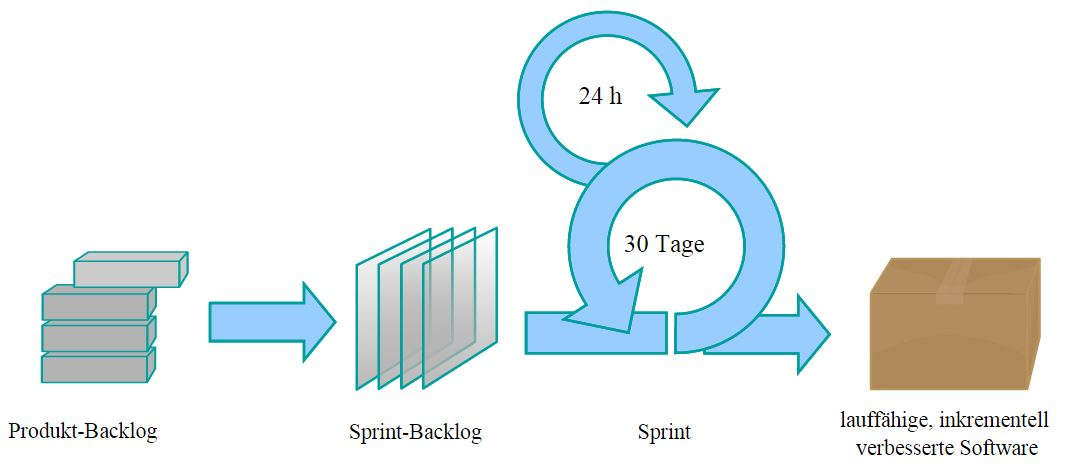
\includegraphics[scale=0.5]{Images/scrum_prozess}
	\caption[Scrum Prozess]{Der Scrum Prozess\cite{wikipedia:scrum}}
	\label{fig:spiralmodell}
\end{figure}
Das Scrum Framework definiert 3 Rollen, 3 Artefakte und 5 Aktivitäten.

\section{Scrum Rollen}
\label{sec:scrum_rollen}
Es gibt 3 Scrum Rollen: Product Owner, Entwicklungsteam und Scrum Master. Die Gesamtheit dieser drei Rollen bezeichnet man als Scrum Team.
\subsection{Product Owner}
Der Product Owner ist sozusagen der Koordinator des gesamten Projekts. Er ist für den wirtschaftlichen erfolg des Projekts und die Ausführung im generellen verantwortlich. Er legt fest welche Funktionen im jeweiligen Spring implementiert werden sollen und priorisiert diese. Der Product Owner ist außerdem für das Product Backlog verantwortlich und aktualisiert dieses auf regelmäßiger Basis. Außerdem ist er die zentrale Kommunikationsschnittstelle zwischen Auftraggeber und Auftragnehmer.
\subsection{Entwicklungsteam}
Das Entwicklungsteam ist dafür verantwortlich, die im Produkt Backlog bzw. in weiterer Folge im Sprint Backlog spezifizierten Funktionen umzusetzen.
Das Entwicklungsteam organisiert sich dabei eigenständig. Die Entscheidung wie und in welcher Reihenfolge die Backlogeinträge umgesetzt werden obliegt einzig und allein den Mitgliedern des Entwicklungsteams.
Entwicklungsteams haben meist eine Größe von drei bis 9 Mitgliedern, wobei allerdings darauf geachtet wird das Team möglichst klein zu halten, da sonst der Koordinationsaufwand steigt.
\subsection{Scrum Master}
Der Scrum Master kümmert sich um die fehlerfreie Ausführung des gesamten Scrum-Prozesses. Er arbeitet eng mit dem Entwicklungsteam zusammen, gehört diesem jedoch selbst (meistens) nicht an. Der Scrum Master ist nicht der Vorgesetzte des Entwicklungsteam, er versteht sich vielmehr als Coach, welcher dem Team bei Problemen diverser Art beisteht und zur Behebung dieser beiträgt. Zu den Aufgaben des Scrum Masters gehören auch das moderieren von Treffen und die Überprüfung der Einhaltung der Scrum Regeln.

\section{Artefakte}
\subsection{Product Backlog}
Unter Product Backlog wird die Auflistung aller vom Kunden gestellten Anforderungen an das Projekt verstanden. Es ist dynamisch, wird also nicht nur einmal erstellt und dann abgearbeitet sondern wird auf regelmäßiger Basis weiterentwickelt. Der Product Owner ist für das Product Backlog der alleinige verantwortliche. Er kümmert sich unter Anderem auch um die Priorisierung der Backlogeinträge.
Die Kundenanforderungen im Product Backlog werden soweit möglich nicht in technischner Fachsprache, sondern anwendungsorientiert und fachlich als User Stories definiert.
\subsection{Sprint Backlog}
Der Sprint Backlog ist, ähnlich wie der Product Backlog, eine Auflistung der Anforderungen. Im Sprint Backlog werden allerdings nur einige wenige Einträge des Product Backlogs übernommen, die für den aktuellen Sprint anfallen. 
\subsection{Product Increment}
"Das Inkrement ist die Summe aller Product-Backlog-Einträge, die während des aktuellen und allen vorangegangenen Sprints fertiggestellt wurden. Am Ende eines Sprints muss das neue Inkrement in einem nutzbarem Zustand sein und der Definition of Done entsprechen."\cite{wikipedia:scrum}

\section{Aktivitäten}
\subsection{Sprint Planning}
Im Sprint Planning spielen zwei essentielle Fragen eine Rolle:
\begin{itemize}
	\item Was kann im kommenden Sprint entwickelt werden?
	\item Wie wird die Arbeit im kommenden Sprint erledigt?
\end{itemize}
Das Sprint Planning dauert in Summe maximal 2 stunden pro Sprint Woche.
Der Product Owner stellt dem Entwicklungsteam die definierten einträge des Product Backlogs vor. Zunächst arbeitet das gesamte Team daran, die festgelegten Backlogeinträge zu verstehen und die Arbeit einzuteilen.
Es werden auch die Akzeptanzkriterien festgelegt, welche am Ende des Sprints darüber entscheiden ob das neue Inkrement der "Definition of Done" entspricht, also fertig ist. In weiterer Folge wird der Aufwand abgeschätzt und die Anzahl der Product Backlog Einträge, welche in diesem Sprint erledigt werden können wird festgelegt. Über die Reihenfolge und Priorisierung der Einträge entscheidet dabei der Product Owner alleine.
In weiterer Folge wird dann im Detail geplant, welche Tasks zur Erfüllung der Product Backlog Einträge notwendig sind.
Das Ergebnis des Sprint Plannings ist der Sprint Backlog
\subsection{Daily Scrum}
Der Sinn des Daily Scrum ist, dass sich alle Teammitglieder einmal am Tag zu einem kurzen, maximal 15 Minuten langen, Meeting zusammenfinden. Dabei sollen allerdings nicht Probleme und auftretende Bugs besprochen werden, sondern ein aktiver Informationsaustausch stattfinden. Jedes Teammitglied gibt kurz und bündig eine Übersicht über den Status der aktuell bearbeiteten Tasks. so weiß jedes Mitglied des Entwicklungsteams immer genau über den Status der anderen Mitglieder bescheid.
Product Owner und Scrum Master sind beim Daily Scrum zwar häufig anwesend, beteiligen sich aber nicht aktiv am Gespräch.
\subsection{Sprint Review}
Das Sprint Review findet am Ende eines jeden Sprints statt. Dabei wird überprüft ob das Team die zu Beginn im Sprint Planning festgelegten Ziele erreicht wurden. Am Sprint Review nehmen zusätzlich zum Scrum Team auch die Steakholder Teil und es wird besprochen wie die weitere Vorgehensweise aussieht. Weiters ist es von Vorteil wenn auch Kunden und Anwender an diesen Besprechungen teilnehmen, da diese die Funktionalität bzw. bedienbarkeit des fertigen Inkrements am besten beurteilen können.
\subsection{Sprint Retrospektive}
Die Sprint Retrospektive findet, ebenso wie das Sprint Review, am Ende eines Sprints statt. Im Gegensatz zum Sprint Review, nehmen daran allerdings nur Mitglieder des Scrum Teams teil. Steakholder können in manchen fällen nur auf Einladung dazu kommen. Das Team überprüft seine Arbeitsweise auf kritische Art und Weise, daher müssen auch unangenehmen Wahrheiten offen geäußert werden. In weiterer Folge werden dann Verbesserungsvorschläge festgelegt und dokumentiert.
\subsection{Product Backlog Refinement}
Als Product Backlog Refinement bezeichnet man den laufenden Prozess, bei dem der Product Owner zusammen mit dem entwicklungsteam den Product Backlog akutalisiert bzw. weiterentwickelt.
Es gibt eine Reihe von Aktivitäten, welche zum PBR gehören, unter Anderem:
\begin{itemize}
	\item Ordnen von Einträgen
	\item Löschen von einträgen die nicht mer benötigt werden
	\item Hinzufügen von neuen Einträgen
	\item Planung von Releases
	\item Detaillieren von Einträgen
\end{itemize}
Da die Steakholder Wertvolle Informationen und Anmerkungen für das Produkt bzw. das Product Backlog liefern können, finden meistens regelmäßig auch sogenannte Product-Backlog-Refinement-Meetings zusammen mit ausgewählten Stakeholdern statt.

\chapter{Feature Driven Development}
Feature Driven Development\footnote{Abk.: FDD} ist ein Vorgehensmodell, dass auch zur agilen Softwareentwicklung. Es ist ein Set an Arbeitstechniken, Strukturen, Rollen und Methoden für das Projektmanagement von Software Projekten.
\paragraph*{}
FDD wurde ursprünglich als schlanke, einfache Methode ein zeitkritisches Softwareprojekt durchzuführen. Dabei soll der Begriff "Feature" im Mittelpunkt. Jedes Feature das entwickelt wird, stellt einen Mehrwert für das Projekt und infolgedessen auch für den Kunden dar. 
Die Planung findet anhand eines Feature-Plans statt. 
\paragraph*{}
Bei FDD gibt es 2 wichtige Rollen:
\begin{itemize}
	\item \textbf{Der Chefarchitekt (Chief Architect)} \newline
		Er behält den Überblick über die gesamtarchitektur des Projekts und die fachlichen Kernmodelle.
	\item \textbf{Der Chefprogrammierer (Chief Programmer)} \newline
		Er führt das Entwicklerteam an und behält die Übersicht über die Aufgaben der einzelnen Programmierer. Bei größeren Projekten können auch mehrere Entwicklerteams mit je einem Chefprogrammierern.
\end{itemize}
\section{Vorgehensweise}
FDD definiert füf zentrale Prozesse:
\begin{figure}[h]
\centering
	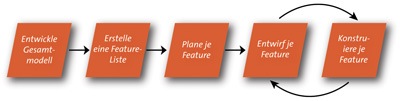
\includegraphics[scale=1]{Images/fdd_prozesse}
	\caption[FDD-Prozesse]{Die FDD Prozesse\cite{wikipedia:fdd}}
	\label{fig:fdd}
\end{figure}
Die Prozesse 1-3 werden innerhalb weniger Tage durchgeführt, 4 und 5 werden allerdings ständig wiederholt

\chapter{Simultaneous Engineering}



\chapter{Rational Unified Process}


\chapter{Aufgabenstellungen}
\section{Frage 1}
Ihre Firma möchte ein Softwareprojekt im kleinen Rahmen beginnen, als ranghoher Mitarbeiter mit Erfahrung im Projektmanagement, wurden Sie damit beauftragt ein passendes Vorgehensmodell auszuwählen. Geben Sie einen Überblick über die gängigsten Vorgehensmodelle und stellen Sie insbesondere den Nachteil klassischer Phasenmodelle dar.
\section{Frage 2}
Sie arbeiten als Projektleiter an einem Softwareprojekt, welches zum jetzigen Zeitpunkt mit dem klassischen Wasserfallmodell durchgeführt wird. Da das Projekt nach einem kritischen Fehler in der Design-Phase neu gestartet werden muss, empfehlen Sie dringlich Scrum als Vorgehensmodell einzusetzen, Ihr Vorgesetzter ist allerdings von den Vorteilen des Wasserfallmodells überzeugt. Stellen Sie den Vorteil von agiler Softwareentwicklung in Form von Scrum im Gegensatz zum Wasserfallmodell dar.
\section{Frage 3}
Ihre Firma hat gerade eine Ausschreibung 

\nocite{*}
\printbibliography

\listoffigures

\end{document}